\documentclass[12pt]{article}
\usepackage[a4paper, total={7.5in, 10in}]{geometry}
%\usepackage{array}

\usepackage[siunitx, RPvoltages]{circuitikz}
\usepackage{graphicx, subfig, wrapfig, fancyhdr, lastpage, multicol ,color,mhchem}
\newcommand\headerMe[2]{\noindent{}#1\hfill#2}
\usepackage[mathscr]{euscript}

\setlength{\columnseprule}{1pt}
\def\columnseprulecolor{\color{blue}}


\pagestyle{fancy}
\fancyhf{}

\cfoot{\em{Page \thepage \hspace{1pt} / \pageref{LastPage}}}
\begin{document}

\headerMe{Royaume du Maroc}{année scolaire \emph{2021-2022}}\\
\headerMe{Ministère de l'Éducation nationale, }{  Professeur :\emph{Zakaria Haouzan}}\\
\headerMe{du Préscolaire et des Sports}{Établissement : \emph{Lycée SKHOR qualifiant}}\\

\begin{center}
Devoir Surveillé  N°3 \\
    Filière 1Bac Sciences Expérimentales\\
Durée 2h00
\\
    \vspace{.2cm}
\hrulefill
\Large{Chimie 7pts/42min}
\hrulefill\\

    %\emph{Les questions parties sont indépendantes}
\end{center}
%end Headerss------------------------
%__________________Chimie ______________________-
%%%%%%%+_+_+_+_+_+_+_+_+_Partie1

 \section*{Partie 1 :Titrage conductimétrique \dotfill(7pts) }

\begin{wrapfigure}[7]{r}{0.4\textwidth}
  \begin{center}
    \vspace{-1cm}
    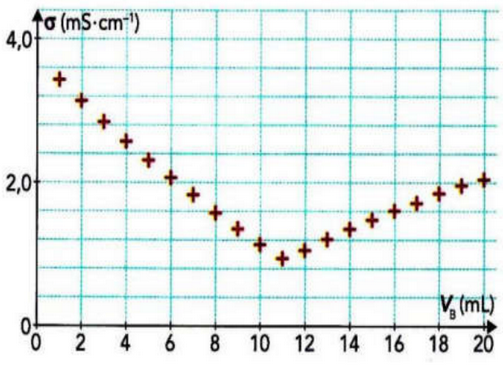
\includegraphics[width=0.3\textwidth]{./img/Screenshot from 2022-05-11 17-55-37.png}
  \end{center}
\end{wrapfigure}
Pour déterminer la concentration $C_1$ de la solution (S1) de sulfate de fer II $({Fe^{2+}}_{(aq)} + {SO_4^{2-}}_{(aq)})$, on dose un volume $V_1=25 mL$ de la solution(S1) par une solution (S2) de permanganate de potassium $(K^+ + MnO_4^-)$ de concentration $C_2=0,1 mol/L.$
 
 Le suivi du titrage par conductimétrie permet de tracer le graphe $\sigma = f(V_B)$ ci-dessous :

Données : - Couples oxydant / réducteur mis en jeu :\\ $Fe^{3+}/Fe^{2+}$ et $MnO_4^-/Mn^{2+}$.
\begin{enumerate}
  \item  Faire un schéma légendé du dispositif de titrage.\dotfill(1pt)
  \item Etablir l’équation de la réaction de dosage.\dotfill(1pt)
  \item Etablir un tableau d’avancement.\dotfill(1pt)
  \item Déterminer la relation d’équivalence.\dotfill(1pt)
  \item Déterminer la concentration C1 de la solution (S1).\dotfill(1.5pt)
  \item  On se place maintenant après l'équivalence.
    \begin{enumerate}
      \item  Quel est le réactif limitant?\dotfill(0.25pt)

      \item  Établir l'expression de la conductivité $\sigma$ \dotfill(0.25pt)

   \item Justifier l'évolution de la conductivité de la solution
     contenue dans le bécher après l'équivalence du titrage.\dotfill(0.25pt)
    \end{enumerate}

  \item  On se place avant l'équivalence.
    \begin{enumerate}
      \item  Quel est le réactif limitant?\dotfill(0.25pt)

      \item  La concentration en ions Sulfate  varie-t-elle au cours du
        titrage?\dotfill(0.25pt)
       
      \item  Établir l'expression de la conductivité $\sigma$ \dotfill(0.25pt)

    \end{enumerate}
\end{enumerate}

 %_____________________________________PHYSIque Partie 22222____________________________________________________________________________
\begin{center}
    \vspace{3.5cm}
\hrulefill
\Large{Physique 13pts - 78min}
\hrulefill\\
    %\emph{Les parties sont indépendantes}
\end{center}
%end Headerss------------------------
 \section*{Partie 1 :Champ magnétique créé par un courant électrique  \dotfill(13pts)}

  On considère une bobine de rayon $R=3cm$ et de longueur $L=60cm$ composée de $N=900$ spires et parcourue par un courant électrique d'intensité $I=300mA$ comme l'indique la figure (2).

\begin{enumerate}
   \item Donner la définition d'un solénoïde.\dotfill(1pt)

   \item  Déterminer l'intensité du champ magnétique crée par ce solénoïde.\dotfill(1pt)

   \item Préciser la nature de chacune des faces du solénoïde et Préciser les pôles de l'aiguille aimantée.\dotfill(1pt)

   \item  Déterminer le sens et la direction du champ magnétique $\vec{B}$ créé par le solénoïde à l'intérieur.\dotfill(1pt)

  \item Représenter le spectre du champ magnétique créé par le solénoïde.\dotfill(1pt)

  \item Sachant que le diamètre du fil enroulé d=3mm, quelle est le nombre de couches enroulées sur le cylindre formant le solénoïde\dotfill(1pt)
  \begin{center}
     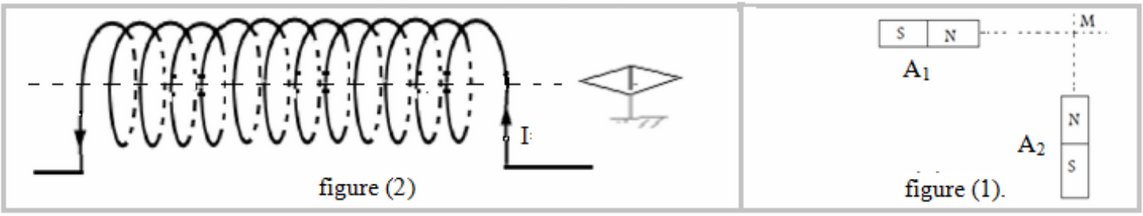
\includegraphics[width=0.85\textwidth]{./img/Exo__sol.png}
  \end{center}

\item On considère deux barreaux aimantés $A_1$ et $A_2$ posés sur le même alignement avec un point M comme l'indique la
figure (1). Sachant que les intensités des champs magnétiques créés par A1 et A2 au point M sont : $B_1=20mT$ et $B_2=30mT$.
    \begin{enumerate}

      \item Représenter les vecteurs champ magnétique en utilisant l'échelle suivante $1cm ->10mT$.Puis représenter le vecteur champ magnétique globale au point M.\dotfill(2pt)

\item Déterminer graphiquement puis par calcul l'intensité du champ magnétique 
  global au point M, puis déterminer l'angle que forme $\vec{B}$ avec le plan horizontal.(On néglige le champ magnétique terrestre.)\dotfill(2pt)
    \end{enumerate}
  \begin{center}
     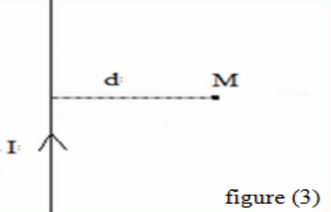
\includegraphics[width=0.2\textwidth]{./img/Exo_fil.png}
  \end{center}


   \item  On considère un long conducteur rectiligne parcouru par un courant électrique d'intensité I=12A comme l'indique la
figure (3) :
    \begin{enumerate}
      \item Donner l'expression du champ magnétique créé par le conducteur au point M\dotfill(1pt)

      \item Représenter Le vecteur champ magnétique créé par le conducteur au point M.\dotfill(1pt)


      \item Calculer l'intensité du champ magnétique créé par le conducteur au point M on donne d=2m\dotfill(1pt)
    \end{enumerate}
\end{enumerate}
\end{document}
